\chapter{Résumé détaillé}

\selectlanguage{french}

\section{Introduction : robots, interaction et connaissances}
\label{chapt|introduction}

Nao a été aperçu jouant avec des enfants autistes, Justin tapote sur la boite
de chocolat en poudre pour préparer le petit-déjeuner, des robots PR2 nous
amènent des bières et distribuent du popcorn dans les laboratoires, tandis que
Rosie s'occupe des crêpes pour le goûter : si ces expériences récentes, mises
en place un peu partout dans les laboratoires de robotique nous dise une chose,
c'est que la robotique de service est en train de quitter le domaine de la
science-fiction, des rêves, des fantasmes et s'apprête à frapper à la porte de
notre quotidien.

\begin{figure}[!h]
    \centering
    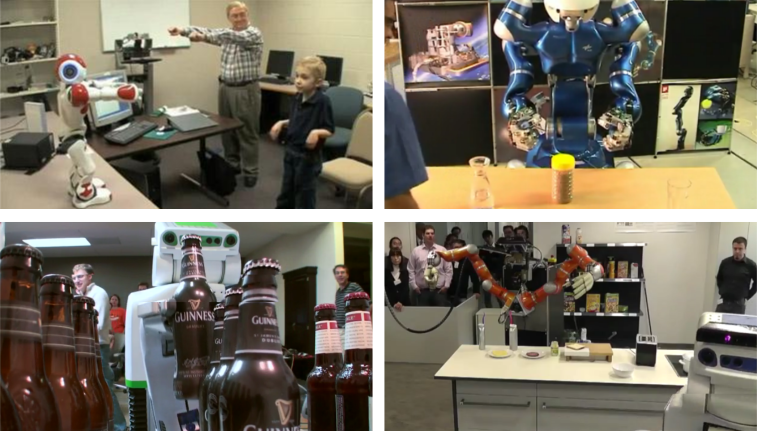
\includegraphics[width=0.8\columnwidth]{intro/everyday_robots.pdf}

    \caption*{Nao, Justin, PR2, Rosie: les robots jouent avec les enfants,
    préparent des chocolats chauds, décapsulent les bières et font sauter les
crêpes. Pour l'instant en laboratoire, sans interactions très avancées avec les
hommes. Que leur manquent-ils pour s'inviter dans nos maisons ?}

    \label{fig|everyday-robots}
\end{figure}

Des progrès considérables ont été accomplis au niveau de la perception des
robots : les caméras et les lasers sont aggrégés dans des pseudo-capteurs
renvoyant des informations de haut-niveau : reconnaissance de visages,
localisation et cartographie SLAM, posture dynamique des hommes... Permettre à
un robot de comprendre son environement est aujourd'hui un défi où deux
facettes se mèlent : reconstruire en continu un monde géométrique et dynamique
cohérent ; abstraire ce même monde en une représentation symbolique adaptée au
raisonnement logique.

La résolution de ce premier défi, auquel cette thèse tente de contribuer, n'est
cependant pas suffisante pour permettre une interaction entre hommes et robots.
Le robot auquel nous pensons vit dans le monde réel, un monde pour et avec des
humains. Notre robot doit acquérir des compétences sociales, il doit pouvoir
considérer les hommes autour de lui non seulment comme des entités physiques
(...sur lesquelles ils ne faut pas rouler par exemple), mais aussi et surtout
comme des entités intelligentes, dotées d'une individualité propre et unique.

Le robot doit pouvoir non seulement représenter son environement, représenter
son propre état mental, mais aussi tenter de deviner et de représenter l'état
mental, les connaissances des autres agents avec lesquels il interagit. Et ces
modèles, il faut ensuite savoir les mettre en \oe uvre pour donner corps  des
compétences sociales au premier rang desquelles se trouve la fonction de
communication.

\subsection{Un programme}
\label{sect|challenges}

Cette brève introduction laisse deviner en négatif le programme de recherche que nous
défendons dans cette thèse, et que nous résumons ici. Nous pouvons essayer
d'articuler les trois défis liés au champ de la représentation des
connaissances dans la robotique de service et robotique-compagnon que nous
traitons dans ce travail de doctorat.

Notre premier objectif est en réalité de préciser cette notion de
\emph{représentation de la connaissance} qui est en réalité mal définie. Depuis
l'enfance de l'intelligence artificielle, depuis l'idée de \og  l'étage de la
connaissance \fg de Newell, il est admis que les systèmes intelligents ont
besoin de représenter et de manipuler de la connaissance. Mais quoi au juste ?
Il semble nécessaire de poser des fondations théoriques et pratiques solides à
cette question sur lesquelles le champ de la robotique cognitive pourrait
s'appuyer. C'est notre premier défi.

Le deuxième défi est plus technique : comment effectivement réaliser un tel
robot cognitif ? quelles sont les spécificités de la robotique (notament du
fait de l'incarnation physique du robot) ? pouvons nous aujourd'hui construire
au moins une instance d'un système cognitif adapté à l'interaction dans le
monde physique ?

Notre troisième défi se concentre sur les aspects liés à l'interaction
homme-robot. Nous affirmons que les robots appartiennent désormais à l'ensemble
des individus sociaux. Qu'est-ce que cela signifie ? quelles conséquences cela
a-t'il sur notre modèle de connaissances ? comment cela se traduit-il en
problèmatique concrète comme la compréhension du language naturel ?

Chacunes des contributions de cette thèse, résumées ci-dessous, peuvent être
rapportées à l'un de ces défis, et nous espérons qu'elles contribuent à une
meilleure compréhension de ces problématiques.

%%%%%%%%%%%%%%%%%%%%%%%%%%%%%%%%%%%%%%%%%%%%%%%%%%%%%%%%%%%%%%%%%%%%%%%%%%%%%%%

\subsection{Contributions de cette thèse}
\label{sect|contributions}

Le point de départ de cette thèse est le sentiment qu'une meilleure
compréhension des besoins en terme de connaissance des applications robotiques
en environement humain (c'est à dire, complexe, dynamiques et sémantiquement
riche) serait bénéfique à la recherche en robotique cognitive.

Se basant sur une large revue de la littérature et la formulation de plusieurs
scénarios d'interaction (dont certains ont conduit a des expériences sur les
robots), nous avons itérativement affiné la problématique de la
\emph{connaissance pour l'interaction}. La formalisation de cette problématique
est l'un des principaux résultats de ce travail : nous avons listé et organisé
en une typologie un ensemble de caractéristiques souhaitées des systèmes de
représentation de connaissance pour la robotique de service.

Cette typologie vise à proposer une base complète et cohérente pour évaluer les
systèmes existants et tirer de nouvelles perspectives de recherche. Elle aide
aussi à évaluer les progrès de la communauté scientifique en direction de
l'objectif long terme d'une intelligence artificielle de niveau humain, pour
reprendre les mots de McCarthy.

Une autre contribution scientifique de cette thèse est liée au rapprochement
des recherches entre les agents intelligents non-incarnés (virtuel) et incarnés
: nous avons essayé de jeter de nouveaux ponts entre des années de recherche
sur les architectures cognitives désincarnées (aussi bien en informatique qu'en
neuropsychologie) et les contraintes des systèmes réels qui pèsent sur les
architectures robotiques. En particulier, nous avons essayé d'identifier un
certain nombre de contributions théorique en sciences cognitives pertinentes
pour la robotique cognitive, et nous avons proposés, pour certaines fonctions
cognitives, des implémentations de références sur les robots.

Au niveau architectural, notre travail aide aussi à mieux comprendre les flux
de connaissances dans des architectures de robotique cognitive modernes. En
explicitant la connaissance, nous la rendons en quelque sorte \emph{palpable},
et nous permettons aux humains qui conçoivent et programment les robots de
discuter et de remettre en question cette connaissance. Ceci singularise et
matérialise des concepts qui étaient auparavant souvent diffus et ubiquitaires.
Cela nous amène à définir et proposer l'idée d'une architecture \emph{orientée
connaissance}.





This work has also several more focused scientific contributions. The
centralised semantic architecture that we propose is original. While it
exhibits shortcomings for some cognitive tasks, it also proposes novel
efficient ways to represent and manipulate knowledge simultaneously for
multiple agents (chapter~\ref{chapt|oroserver}). Along with the survey of
current knowledge systems that we have conducted, it effectively completes the
picture of available designs of knowledge representation systems.

Amongst the cognitive abilities that our developments have enabled, a
particular scientific focus was led on the acquisition and modeling of
multiple, agent-dependent symbolic worlds. This opened new perspectives related
to \emph{perspective-aware} reasoning or \emph{theories of mind} for robots
that are detailed in this work.

We also have a scientific contribution on the grounding of human-robot dialogue
in natural language (chapter~\ref{chapt|dialogs}). We have algorithmically
formalised a grounding process that takes advantage of multi-modal
communication (verbal, deictic and immanent) and handles the semantics of
several more complex language features like quantification. This system also
has contributions related to the semantic validation of thematic roles and
interactive disambiguation that takes into account human attentional focus.

\subsection{Technical contributions}
\label{sect|technical-contributions}


This thesis has four major technical contributions: the software development of
the \emph{ORO server} as a semantic blackboard dedicated to robotic
applications, the design of the \emph{ORO ontology} as a domain-specific
common-sense ontology tailored for service robotic needs, the pervasive
integration of a new semantic layer into several existing robot architecture,
and finally, the software development of \emph{Dialogs}, a module for natural
language grounding.

The main software contribution of the thesis is the development of an
open-source, versatile and light-weight knowledge base that stores in a formal
framework based on first-order logics both the robot's own beliefs and the
mental models (as perceived by the robot) of every other cognitive agent that
the robot interacts with (chapters~\ref{chapt|oroserver}
and~\ref{chapt|implementation-integration}).  This tool, called \emph{ORO}, is
implemented as a platform/middleware-agnostic server, and exposes to the
robot's modules several advanced reasoning services (via the integration of
external reasoners). This software project is now publicly available, used by
other laboratories, and comes with extensive documentation and bindings for
several mainstream languages (C++, Python...) and middleware (ROS, YARP).

In parallel of this development, and in collaboration with other developers, we
have also drafted (and partially implemented) a proposal for a standard API for
knowledge manipulation that supports the specific needs of robotic applications
(section~\ref{sect|knowledge-api}).

Coming along with the ORO server, we introduce in this thesis the \emph{ORO
common-sense ontology} which is a proposal of an upper ontology for service and
interactive robotics (section~\ref{sect|oro-commonsense}). This ontology
consists of about two hundred classes, relations and rules that are relevant
for the modeling of the robot's beliefs and state, and the interactions with
other agents (humans or robots). This ontology also tries to stay closely
aligned with the standard {\sc OpenCyc} upper-ontology to guarantee
interoperability with semantic web resources and other robots.

A third technical contribution is the introduction of a new knowledge-oriented,
event-driven communication model between high-level decisional modules
(section~\ref{sect|integration}): by introducing the notion of \emph{semantic
events}, the ORO server enables the development of new executive layers that
combine reactive behaviour with high-level abstractions: for instance,
triggering a behaviour when a human looks at the robot while sit, can be
expressed in our architecture as a single proposition: {\tt subscribe([* type
Human, * looksAt myself, * isSitting true], behaviour\_callback())}. This
highly expressive event model opens a new range of development opportunities for
decisional modules.

During the preparation of the thesis, we have also developed a new stand-alone
natural language processor for English language (chapter~\ref{chapt|dialogs}).
It takes advantage of the different symbolic models exposed by the ORO server
to analyse, resolve the semantics and ground dialogues. It can process orders,
questions and positive assertions and translates them into new symbolic facts.
It includes a custom grammatical parser, a re-verbalization module, several
discrimination strategies, including interactive ones. The application is
developed in Python (about 15K lines of code), can be used in real-time on the
robot, and is accompanied by a speech recognition interface developed as an
Android application.

A last notable software contribution is our involvement in the MORSE simulator
for academic robotics. We have played a central role in the original design and
development of the core functionalities of this open-source simulator which is
now used by over twenty laboratories world-wide. While this project as a whole
is not directly related to main topic of the thesis, we have led the effort
towards effective simulation of human-robot interaction in MORSE. It is briefly
presented at section~\ref{sect|simulation}.



%%%%%%%%%%%%%%%%%%%%%%%%%%%%%%%%%%%%%%%%%%%%%%%%%%%%%%%%%%%%%%%%%%%%%%%%%%%%%%%
%%%%%%%%%%%%%%%%%%%%%%%%%%%%%%%%%%%%%%%%%%%%%%%%%%%%%%%%%%%%%%%%%%%%%%%%%%%%%%%
%%%%%%%%%%%%%%%%%%%%%%%%%%%%%%%%%%%%%%%%%%%%%%%%%%%%%%%%%%%%%%%%%%%%%%%%%%%%%%%

\section{Robots for interaction}
\label{sect|hri-context}

This work comes indeed from researches in the specific context of the
human-robot interaction, or, to put it another way, in the context of
interaction for \emph{joint action} with humans,  in a \emph{situated}
environment (figure~\ref{fig|hri-dec}).


\begin{figure}
    \centering
    \includegraphics[width=0.9\columnwidth]{intro/grounding_robot.pdf}
    
    \caption{A robot reasoning about human-robot interaction and anticipation
    of human activities: sources of knowledge are multi-modal dialogue and
    observation of the environment and the human activities. The robot ``knows''
    and reasons about the fact it is observed by the human.}

    \label{fig|hri-dec}
\end{figure}



{\em ``\emph{Let's bake a brownie for tonight!}'', proposes Tom. The robots
smoothly prepare all the ingredients, and they start to cook together a
delicious cake...}

Natural interaction and cooperation are actually the current (dare we say,
\emph{short-term}) targets for the human-robot interaction community.  The
``Brownie scenario'' we presented above belongs to the broad class of
\emph{interactive manipulation problems}: several agents agree on a (more or
less implicit) joint goal that requires some sort of cooperation to be
successfully achieved. This class of problems involves both dialogue and
manipulation and they are often not completely defined at start-up: they require
iterative, interactive resolution (step-by-step process,
questions-answers,...).

What are the cognitive prerequisites for such a sentence --``Let's make a
brownie for tonight''-- to be understood by the robot, correctly interpreted in
the spatial and temporal context of the interaction, and eventually transformed
into a set of actions? We distinguished four main tasks in~\cite{Lemaignan2012}:

\begin{enumerate}

    \item building and maintenance of a consistent geometric model of the
        current situation, acquired through perception or deduction from
        previous perceptions,

    \item building of an unambiguous and complete symbolic representation of
    concepts (objects, agents, actions...) underlying the interaction, and
    practical for decision-making processes,

    \item establishing the joint goal(s), building and maintenance of
        iteratively shared (human-robot) plans, 

    \item refinement and execution of the computed plans, and monitoring of
        those achieved by the human partner.

\end{enumerate}

While each of these items is equally important to actually perform the
interaction -- and we will present (with illustration from experiments) how our
knowledge representation system integrates and communicates with other
processes to form a \emph{knowledge-enabled} robotic architecture --, the
thesis focuses on the second point: it presents techniques, developed and used
on several real robots, for the symbolic representation of environment and
mental models suitable for grounded situation interpretation, decision-making
and control.

\paragraph{Models for the interaction} Figure~\ref{fig|hri-dec} summarises the
main aspects of the interaction, that are to be translated into models.  From
the robot perspective, several cognitive skills are involved: dialogue
processing through verbal and deictic modalities (what does the human say? What
attitude -- gaze orientation, postures, gestures... -- does he express?), acquisition
and maintenance of one or several models of the environment, not only from the
robot point of view, but also from the other agents' points of view,
anticipation (what are the intentions of the human? Can I predict and
anticipate his/her actions?), planning and control (how would I proceed further
towards the goal?), monitoring of the other agents' activities (do we have an
effective cooperation?) and the overall progress of the task. 

As we shall see, all these cognitive capabilities also translate into
requirements on the knowledge representation systems that we want to clarify.

%%%%%%%%%%%%%%%%%%%%%%%%%%%%%%%%%%%%%%%%%%%%%%%%%%%%%%%%%%%%%%%%%%%%%%%%%%%%%%%


%%%%%%%%%%%%%%%%%%%%%%%%%%%%%%%%%%%%%%%%%%%%%%%%%%%%%%%%%%%%%%%%%%%%%%%%%%%%%%%
%%%%%%%%%%%%%%%%%%%%%%%%%%%%%%%%%%%%%%%%%%%%%%%%%%%%%%%%%%%%%%%%%%%%%%%%%%%%%%%
%%%%%%%%%%%%%%%%%%%%%%%%%%%%%%%%%%%%%%%%%%%%%%%%%%%%%%%%%%%%%%%%%%%%%%%%%%%%%%%
\section{Symbolic Knowledge Representation}


In that chapter, we have first discussed a definition of \emph{knowledge} in
our context of service robotics and human-robot interaction. We have presented
several references from the literature regarding the identification and
classification of prominent features of knowledge representation systems. 

We have then introduce a comprehensive typology of such features, that
comprises of about fifty concepts sorted into six main categories: features
related to knowledge expressiveness, features related to representation
techniques, features related to reasoning, features related to acquisition and
grounding of knowledge, features related to the integration of a KRS into a
larger robotic architecture, and finally, features that characterise the
represented knowledge itself. Each of the fifty concepts has been briefly
presented with references to the literature.

Finally, we have surveyed eight systems for knowledge representation in service
robots and underlined their main strengths.


\paragraph{What do we call ``knowledge''?}
\label{sect|on-knowledge}

Since we will discuss at length the concept of knowledge in the context of
robotics in the coming pages, it is useful to make our terminology explicit.

Be it in philosophy, cognitive sciences or computer sciences, reaching an
agreement on a definition of ``knowledge'' seems difficult.

Allen Newell's famous \emph{Knowledge Level}~\cite{Newell1981} can be a
starting point: for Newell, \emph{knowledge} is a medium between \emph{agents}
and \emph{goals}, \emph{actions}, \emph{bodies}. Whereas the symbol level deals
with representation, the knowledge level deals with language, semantics;
whereas the symbol level deals with inference, the knowledge level deals with
entailment. We will, at the conclusion of the thesis, give a second look to
this distinction.

In our robotic context, we define knowledge as a narrower concept, while
keeping Newell's link to actions: ``knowledge'' is for us  \emph{a set of
interrelated logical facts that are meaningful to the robot executive
controller}. By \emph{meaningful} we mean that can possibly be interpreted to
lead to a purposeful action. We will see that our main challenge while
designing a cognitive architecture is furthermore to make this knowledge as
\emph{explicit} as possible.


From the perspective of communication, knowledge is for us an information
\emph{interpreted in the cultural and social contexts} of the robot. This
translates into three practical features: knowledge is made of statements that
are \emph{contextualized}, \emph{grounded}, and \emph{limited} to a domain of
validity. These three features have important consequences for the way a
knowledge representation and storage system must be designed.

\section{A typology of knowledge representation requirements for robotics}
\label{sect|features}

This section now focuses on formalizing the knowledge representation issue: we
aim first at establishing a comprehensive typology and nomenclature
(figure~\ref{fig|taxo}) of representational needs for robotics in the specific
context of service robotics, before painting, at
section~\ref{sect|surveyed-systems}, the current landscape of approaches to the
knowledge representation problem in the research community. For each such
``dimensions'' of knowledge representation system, we provide a short
definition accompanied by links to relevant literature.

\begin{figure}
        \centering
        \includegraphics[width=1\columnwidth]{taxonomy.pdf}
        \caption{Taxonomy of the analysis dimensions of knowledge
        representation systems for service robotics.}
        \label{fig|taxo}
\end{figure}

The typology has been built from three main sources: a review of the existing
literature on that topic that we present in the next section; the survey of
eight knowledge representation systems already deployed; our own experience,
acquired during the thesis preparation with the help of many discussions with
researchers from both CNRS and TUM, that allowed to interweave two slightly
different perspectives on knowledge in robotics.

\subsection{What can be represented?}
\label{sect|expressiveness}

This first axis of analysis is its intrinsic expressive power. It answers the
question: what can be possibly represented. When it explicitly exists, the
\emph{language} of representation plays here an obvious role.

%%%%%%%%%%
\subsection{How things are represented?}
\label{sect|higher-level-domain-representation}

We do not discuss in this section the general strategies to construct a
knowledge model (they will be presented in
section~\ref{sect|design-strategies}). We focus here on questions that involve
representational challenges (time, space, context) or require specific
cognitive capabilities (theory of mind, introspection, memory).


\subsection{Reasoning techniques}

\subsection{Acquiring knowledge}

\subsection{Practical integration in robotic architectures}
\label{sect|integration-robot}


Knowledge representation systems do not mean anything to robots if they are
considered in isolation. This section proposes categories of features related
to the integration of the KRS into a larger software architecture that includes
perception routines, decision-making processes and actuation control.

We also mention some practical aspects of a real-world system, like
performances and monitoring tools that come along with the KRS.

\subsection{Knowledge instantiation}

This last branch of our taxonomy looks at the actual \emph{content} of the
knowledge base: the knowledge instantiation. Here, \emph{instantiation} does
not only refer to the instantiation of the knowledge structure (what we have
called the ABox), but also includes the knowledge structure itself (the TBox).

While we have previously mentioned features of knowledge representation systems
that enable the robot to fill its knowledge base with content and alter the
knowledge structure, most of the systems also come with a certain amount of
initial knowledge that often includes \emph{common-sense} knowledge (\ie facts
that widely known to humans, and hence often implicit: ``to put a cake in the
oven, one must first open the oven's door'').

The design strategy, the choice to rely on common-sense knowledge or not, the
reuse of standard ontologies, the quantity of {\it a priori} knowledge are many
parameters that lead to different knowledge models.


\section{Existing systems for knowledge representation in service robotics}
\label{sect|surveyed-systems}


Table \ref{table|surveyed-systems} lists the knowledge representation
systems that we have surveyed.

We have limited ourselves to systems that
\begin{inparaenum} 
    \item  run on \emph{service robot} (that is, robots that interact with 
    objects in a semantic-rich environment primarily designed for humans),
    \item  ground the knowledge in the physical world (physically embedded
    systems able to assess their environment),
    \item  are able to merge different knowledge modalities,
    \item  are able of on-line, dynamic knowledge acquisition and reasoning 
    (\ie not simple static databases).
\end{inparaenum}


\begin{landscape}
\begin{table}\scriptsize
\begin{center}

\begin{tabular}{p{2.2cm}p{1.6cm}p{4cm}lp{2.4cm}p{3.4cm}p{1.5cm}}
\toprule
{\bf Project} & {\bf Category} & {\bf Authors (Institution)} & {\bf Project homepage} & {\bf Programming language} & {\bf Knowledge model/Logical Formalism} & Main reference \\
\midrule
ARMAR/Tapas & Formal & Holzapfel, Waibel \par (Karlsruhe TH) & & & TFS (Typed Feature Structures) & \cite{Holzapfel2008}\\
CAST Proxies & Ubiquitous & Wyatt, Hawes, Jacobsson, Kruijff (Brimingham Univ., DFKI Saarbrücken) & & & Amodal proxies & \cite{Jacobsson2008} \\
GSM & Structural & Mavridis, Roy \par (MIT MediaLab) & & & & \cite{Mavridis2006} \\
Ke Jia Project & Formal & Chen et al. \par (Univ. of Science and Technology of China) & \url{www.wrighteagle.org/en} & ASP (Answer Set Programming) & ASP & \cite{Chen2010} \\
{\sc KnowRob} & Formal & Tenorth, Beetz \par (TU Munich) & \url{ias.in.tum.de/kb/wiki} & {\sc Prolog} & {\sc Prolog} + OWL-DL &  \cite{Tenorth2009a} \\
NKRL & Language & Zarri et al. \par (Paris Est Créteil Univ.) & & NKRL & & \cite{Sabri2011} \\
%OBOC & KRS & Mendoza & & & & & \cite{Mendoza2005} \\
OUR-K/OMRKF & Formal & Lim, Suh et al. \par (Hanyang Univ.) & \url{incorl.hanyang.ac.kr/xe} & ? & DL + Horn Clauses &  \cite{Lim2011, Suh2007} \\
%ORO & KRS & Lemaignan, Alami \par (LAAS-CNRS) & \url{oro.openrobots.org} & {\sc Java} & OWL-DL ({\sc Jena}) & {\sc Pellet} & \cite{Lemaignan2010} \\
PEIS KR\&R & Formal & Daoutis, Coradeshi, Loutfi, Saffiotti \par (Örebro Univ.) & \url{www.aass.oru.se/~peis} & {\sc C}, {\sc CycL} & CycL (1st and 2nd order logics, modal logics) & \cite{Daoutis2009} \\
%Golog & Language & Levesque (Toronto Univ.) & & {\sc Prolog} & & & \\
% & & Varadarajan, Vincze \par (TU Wien) & & & & & \cite{Varadarajan2011} \\ % -> affordances, but no implementation on a robot
% & & Kaelbling, Lozano-Pérez \par (MIT CSAIL) & & & & & \cite{Kaelbling2011} \\ % -> mostly planning under uncertainty
% & & Hertzberg (Osnabrück Univ.) \\ % -> affordances, semantic mapping
% (based on {\sc KnowRob} & & (JSK) \\

\bottomrule

\end{tabular}
\end{center}

\caption{List of surveyed systems. Categories are \emph{Formal} for systems
that have a formal underlying knowledge representation, \emph{Ubiquitous} for
systems where knowledge is fully distributed, \emph{Language} for languages
used as KRS on robots or \emph{Structural} for KRS where knowledge is
represented as special data structures.}

\label{table|surveyed-systems}
\end{table}
\end{landscape}


%%%%%%%%%%%%%%%%%%%%%%%%%%%%%%%%%%%%%%%%%%%%%%%%%%%%%%%%%%%%%%%%%%%%%%%%%%%%%%%
%%%%%%%%%%%%%%%%%%%%%%%%%%%%%%%%%%%%%%%%%%%%%%%%%%%%%%%%%%%%%%%%%%%%%%%%%%%%%%%
%%%%%%%%%%%%%%%%%%%%%%%%%%%%%%%%%%%%%%%%%%%%%%%%%%%%%%%%%%%%%%%%%%%%%%%%%%%%%%%

\section{The OpenRobots Ontology Framework}


We conclude here this third chapter. This chapter was focused on the functional
and algorithmic presentation of the ORO server, a \emph{semantic blackboard}
where robotic modules can write and querying pieces of knowledge.

We have mentioned how multiple mental models can be managed by the server, and
we have also presented several active services, like the discrimination
algorithms or the management of the memory.

Finally, we have presented the ORO \emph{common-sense} ontology that provide
the robot with an initial background knowledge, shared by all the agents.

The next chapter first gives some implementation and technical details about
the ORO framework, and then present how ORO is integrated with other components
on real robots. In particular, we detail the integration with the geometric
reasoning module and the symbolic task planner.



We have adopted a centralised approach for knowledge management called
ORO~\cite{Lemaignan2010}. The platform is designed as a central
knowledge storage service implemented as a server where the robot
components can add or query statements at run-time. Figure~\ref{fig|oro-overview}
illustrates the main functional components of ORO.

\begin{figure}
\centering
  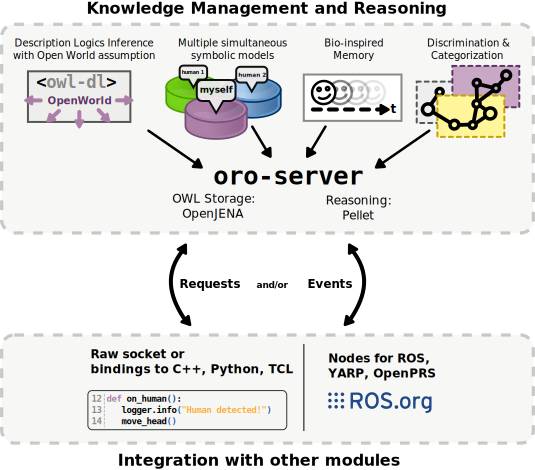
\includegraphics[width=0.75\columnwidth]{oroserver/oro_architecture_functional.pdf}
  \caption{Overview of the ORO architecture.}
  \label{fig|oro-overview}
\end{figure}

At the core, ORO is build around the
OpenJena\footnote{\url{http://www.openjena.org}} ontology management library,
connected to the Pellet\footnote{\url{http://clarkparsia.com/pellet}}
reasoner.

A front-end accepts and manages connections to clients. The clients' requests
are processed by a set of internal modules: basic operations on statements, but
also higher cognitive and human-robot interaction related features are
available. External plugins can also be added via a specific extension
mechanism.

Besides acting as a facts database, the ORO platform exposes several
functions: operations on knowledge statements relying on inference (through a
continuous first-order logic classification process), management of
\emph{per-agent} symbolic models, categorisation of sets of concepts
and profiles of memory (that enable the robot to ``forget'' about some facts).

ORO also provides an event mechanism that allows components to be triggered
when specific events occur. A component can for instance subscribe to events
of kind \setstmt{?agent isVisible true, ?agent type Human}. As soon as the
perception layer detects a human in the robot's field of view and accordingly
updates the knowledge base, the executive layer is triggered. The event
framework also takes advantage of the inference capabilities of ORO. Thus an
event can be indirectly triggered if its triggering conditions can be
inferred to be true.

\subsubsection{Representation of alternative knowledge models}
\label{sect|alterite}

As pictured in Figure~\ref{fig|oro-overview}, ORO stores independent cognitive
models for each agent it interacts with. When the ORO server actually
identifies a new agent (or infers that some instance is an agent), it
automatically creates a new, separate, in-memory OWL model for that agent.
Then, different robot components, like execution control or situation
assessment, may store the agents' beliefs in separate, independent models. All
knowledge processing functions in the robot's primary model are equally
available in every agent's model, which allows us to store and reason on
different (and possibly globally inconsistent) models of the world.

Each of these models is independent and logically consistent, enabling
reasoning on different perspectives of the world that would otherwise be
considered as globally inconsistent (for instance, an object can be visible for
the robot but not for the human. This object can have at the same time the
property \concept{isVisible \textit{true}} and \concept{isVisible
\textit{false}} in two different models).

We present at section~\ref{sect|spark}, page~\pageref{sect|spark}, a 3D
real-time environment, SPARK, that allows to compute on-line several symbolic
properties that are dependent on the perspectives.

\paragraph{Theory Of Mind and contexts} \label{sect|theory-of-mind}

By maintaining independent mental states for each agent it interacts with, we
consider the robot to be endowed with a simple \emph{theory of
mind}~\cite{Scassellati2002}: the robot can explicitly model the beliefs of its
interactors, it expose them to the control architecture, and the same set of
cognitive abilities are available on these secondary model as on the main
model: reasoning, inconsistencies detection, events, etc.

Proper \emph{false beliefs} experiment, similar to the Sally and Ann experiment
presented in the previous chapter, has been recently conducted with ORO
by Mathieu Warnier, as reported in~\cite{Warnier2012a}: in this experiment, two
humans observe a table with several objects, then one leaves while the other
one moves around some objects. This leads to two different set of beliefs on
the world, which the robot explicitly stores and updates when necessary (if the
human comes back and check the table, for instance).

These multiple models can also be viewed as different \emph{interpretive
frames}, allowing the robot to interpret the same reality from different points
of view. In this sense, each model carries a context of interaction.  In
chapter~\ref{chapt|dialogs}, we present how such agent-dependent contexts are
used by a natural language processor to make sense of user sentences from
his/her point of view.

\subsection{Reasoning techniques}

\subsubsection{Standard inference services}
\subsubsection{Grounding, classification and discrimination algorithms}
\subsubsection{Memory}
\subsubsection{Knowledge structure alteration and learning}



\section{Knowledge instantiation: the OpenRobots Common-Sense Ontology}
\label{sect|oro-commonsense}

The ORO platform is made of the server that we have presented, and a
common-sense ontology, the \emph{ORO Common-sense Ontology}.

At start-up, the knowledge model of the ORO server is initialised with a
configurable sets of ontologies that build together the initial pool of facts
known to the robot: the common-sense ontology and optional, domain dependent
ontologies.

Each time a new model is created (typically when a new agent is detected), it
is also initialised with the same pool of facts.  From the point of view of the
robot, this ensure that all the different agents share the same background
knowledge.

Usually, the ORO server is started with the common-sense ontology that we
present in this section, and one scenario-specific ontology that usually
contains the set of individuals with relevant properties needed by the
experiment.

\begin{figure}
    \centering
    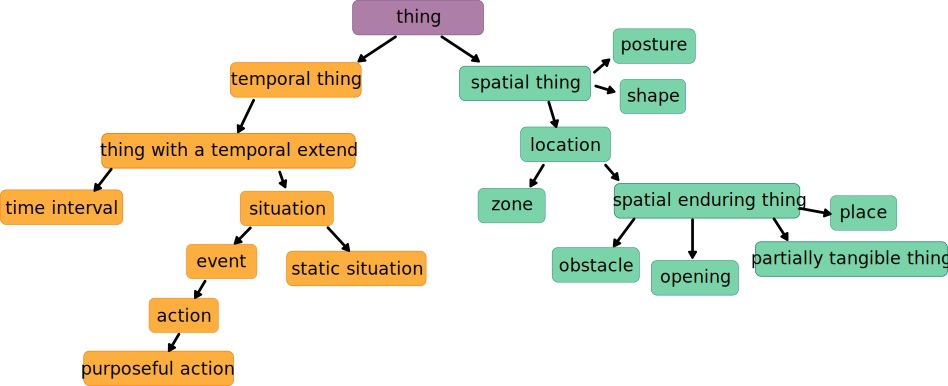
\includegraphics[scale=0.6]{oro/top_tbox.pdf}

    \caption{The upper part of the ORO common-sense TBox. All these concepts
    belong to the {\sc OpenCyc} namespace.}
    
    \label{fig|upper_tbox}
\end{figure}

The ORO common-sense ontology has been designed from two requirements: covering
our experimental needs and conforming as much as possible to the {\sc OpenCyc}
upper ontology.

This lead to a bidirectional design process: from \emph{bottom-up} regarding
the choices of concepts to model, \emph{top-down} regarding the upper part of the
taxonomy. This upper part of the ontology is pictured on
figure~\ref{fig|upper_tbox}. All the classes visible on this figure belong to the
{\sc OpenCyc} namespace (the {\tt cyc:} prefix is omitted).

This figure~\ref{fig|upper_tbox} also illustrates the fundamental disjunction
in the ORO model between \emph{temporal} and \emph{spatial} entities (formally,
$(TemporalThing \sqcap SpatialThing)^{\mathcal{I}} = \emptyset$, with
$\mathcal{I}$ the \emph{interpretation} of our model).

The class \concept{purposeful action} is the superset of all the actions that
are voluntarily performed by the robot (or another agent). Subclasses (like
\concept{Give}, \concept{LookAt}, etc.) are not asserted in the common-sense
ontology, but are added by the execution controller (in link with the symbolic
task planner) and the natural language processor based on what is actually
performable and/or understandable by the robot at run-time.

...mention thqt other pqrts like objects qre much more refined.

Lastly, the ORO common-sense ontology contains several rules and class
expressions that encode non-trivial inferences.

The definition of the \concept{Bottle} is a case in point. We already gave a
simplified version, here the complete definition:

\concept{Bottle} $\equiv$ \concept{Container} {\bf and} \concept{Tableware}
{\bf that} (\concept{hasShape} {\bf value} \concept{cylinderShape} {\bf and}
\concept{hasCharacteristicDimension} {\bf only} \concept{\em int[>= 0.1, <=
0.3]})

If a human informs the robot that a given object is indeed a bottle, the robot
can then infer much more on this object. And if the human affirms that a car is
a bottle, the robot may question this assertion because of the inconsistent
size.

%%%%%%%%%%%%%%%%%%%%%%%%%%%%%%%%%%%%%%%%%%%%%%%%%%%%%%%%%%%%%%%%%%%%%%%%%%%%%%%
%%%%%%%%%%%%%%%%%%%%%%%%%%%%%%%%%%%%%%%%%%%%%%%%%%%%%%%%%%%%%%%%%%%%%%%%%%%%%%%
%%%%%%%%%%%%%%%%%%%%%%%%%%%%%%%%%%%%%%%%%%%%%%%%%%%%%%%%%%%%%%%%%%%%%%%%%%%%%%%
\section{Integration in the robot architecture}
\label{sect|integration}

\begin{figure*}[thpb]
  \centering
  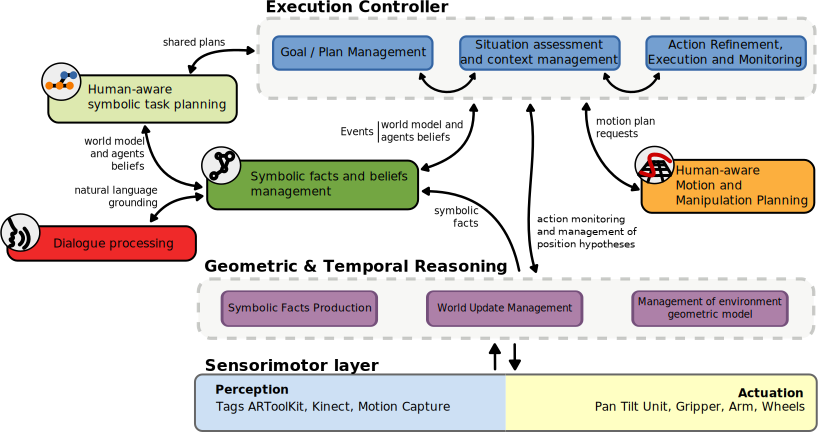
\includegraphics[width=\columnwidth]{integration/architecture_overview.pdf}

  \caption {Software architecture of PR2 and Jido, two service robot
  interacting with humans at LAAS-CNRS.}

  \label{fig|archi}
\end{figure*}

Figure~\ref{fig|archi} presents the organisation of the upper software layer
(the ``decisional'' or ``cognitive'' layer) of the service robots Jido and PR2
as currently in service at LAAS (this architecture is described in detail
in~\cite{Alami2011}). The sensori-motor layer (bottom) is abstracted in SPARK,
an intermediate amodal 3D model where geometric (and some temporal) reasoning
take place.

The outcome of the geometric analysis, as well as the result of the dialogue
processing module ({\sc Dialogs}), are stored in ORO, that plays the role of as
a central knowledge hub. The symbolic knowledge base triggers events that are
captured by a top-level execution controller.

In our architecture, the controller can rely on two specialised planners: MHP,
a geometric motion and manipulation planner~\cite{Sisbot2008, Mainprice2011,
Pandey2010} and HATP, a symbolic task planner~\cite{Alili2009}.

The dialogue processing module, as well as the symbolic task planner, also use
the knowledge base to answer questions or initialise the planning domain.

During a typical interaction experiment (such an experiment is describe at
chapter~\ref{chapt|evaluation}), the execution controller decides upon a goal
to reach, requires a plan from the task planner, allocates the actions to the
human and the robot, communicates the shared plan to the human, and controls
and monitors its execution. The operation continues until the goal is achieved,
is declared unachievable or is abandoned by the human.

In this architecture, only ORO and Dialogs (the dialogue processing module that
we present in the next chapter), as components, are the actual direct outcomes
of this doctoral work. It is however important to present the other one all
here as well since a knowledge base only make sense within a larger
architecture, with knowledge providers and consumers.  Furthermore, the
approach to knowledge management introduced by this thesis had a strong
influence on the design of the communication flows between all these
components. Thus, this section introduces the software components that have
been used in conjunction with ORO (mostly, but not only, on the LAAS robots),
and details how these components produce, exchange and consume symbolic
knowledge.


